\documentclass[
  captions=tableheading,
  bibliography=totoc, 
  titepage=firstiscover,
]{scrartcl}

\usepackage{blindtext} %neuer input

\usepackage{longtable} % Tabellen über mehrere Seiten

\usepackage[utf8]{inputenc} %neuer input

\usepackage{scrhack}

\usepackage[aux]{rerunfilecheck} %Warnung falls nochmal kompiliert werden muss

\usepackage{fontspec} %Fonteinstellungen

\recalctypearea{}

\usepackage[main=ngerman]{babel} %deutsche Spracheinstellung

\usepackage{ragged2e} %neuer input

\usepackage{amsmath, nccmath}

\usepackage{amssymb} %viele mathe Symbole

\usepackage{mathtools} %Erweiterungen für amsmath


\DeclarePairedDelimiter{\abs}{\lvert}{\rvert}
\DeclarePairedDelimiter{\norm}{\lVert}{\rVert}

\DeclarePairedDelimiter{\bra}{\langle}{\rvert}
\DeclarePairedDelimiter{\ket}{\lvert}{\rangle}

\DeclarePairedDelimiterX{\braket}[2]{\langle}{\rangle}{
#1 \delimsize| #2
}

\NewDocumentCommand \dif {m}
{
\mathinner{\symup{d} #1}
}


\usepackage[
  math-style=ISO,
  bold-style=ISO,
  sans-style=italic,
  nabla=upright,
  partial=upright,
  warnings-off={
    mathtools-colon,
    mathtools-overbracket,
  },
]{unicode-math}

\setmathfont{Latin Modern Math}
\setmathfont{XITS Math}[range={scr, bfscr}]
\setmathfont{XITS Math}[range={cal, bfcal}, StylisticSet=1]


\usepackage[
  locale=DE,
  separate-uncertainty=true,
  per-mode=reciprocal,
  output-decimal-marker={,},
]{siunitx}

\usepackage[autostyle]{csquotes} %richtige Anführungszeichen

\usepackage{xfrac}

\usepackage{float}

\floatplacement{figure}{htbp}

\floatplacement{table}{htbp}

\usepackage[ %floats innerhalb einer section halten
  section,   %floats innerhalb er section halten
  below,     %unterhalb der Section aber auf der selben Seite ist ok
]{placeins}

\usepackage[
  labelfont=bf,
  font=small,
  width=0.9\textwidth,
]{caption}

\usepackage{subcaption} %subfigure, subtable, subref

\usepackage{graphicx}

\usepackage{grffile}

\usepackage{booktabs}

\usepackage{microtype} %Verbesserungen am Schriftbild

\usepackage[
backend=biber,
]{biblatex}

\addbibresource{../lit.bib}

\usepackage[ %Hyperlinks im Dokument
  german,
  unicode,
  pdfusetitle,
  pdfcreator={},
  pdfproducer={},
]{hyperref}

\usepackage{bookmark}

\usepackage[shortcuts]{extdash}

%\usepackage{warpcol}


\begin{document}
    \title{V203 Verdampfungswärme}
    \author{  
    Tobias Rücker\\
    \texorpdfstring{\href{mailto:tobias.ruecker@tu-dortmund.de}{tobias.ruecker@tu-dortmund.de}
    \and}{,} 
    Paul Störbrock\\
    \texorpdfstring{\href{mailto:paul.stoerbrock@tu-dortmund.de}{paul.stoerbrock@tu-dortmund.de}}{}
    }
    \date{Durchführung: 17.12.2019, Abgabe: 07.01.2020\vspace{-4ex}}
\maketitle
\center{\Large Versuchsgruppe: \textbf{42}}
    
    \begin{abstract}
    \centering
        \textbf{Ziel:} Bestimmung der Verdampfungswärme von Wasser im Niedrig- und Hochdruckbereich
    \end{abstract}

\newpage
\tableofcontents
\newpage

% Theorie %%%%%%%%%%%%%%%%%%%%%%%%%%%%%%%%%%%%%%%%%%%%%%%%%%%%%%%%%%%%%%%%%%%%%%%%%%%%%%%%%%%%%%%%%%%%%%%%%%%%%%%%%%%%%%%%%%%%%%%%%%%%%%%%%%%%%%%%%%%%%%%%%%%%%%%%%%%%%%%%%%%%%%%%%%%%%%%%%%%%%%%%%%%%%%%%%%

\section{Theorie}\justifying
Bei der Beischreibung von Stoffen wird ihr Aggregatszustand häufig in drei 
Phasen unterteilt: fest, flüssig und gasförmig. 
Für die Zuordnung eines Stoffes in einen bestimmten Aggregatszustand spielen
Druck und Temperatur sowie Stoffeigenschaften eine wichtige Rolle.
Durch ein Zustandsdiagramm lässt sich dies verdeutlichen:
\begin{figure}[H]
    \centering
    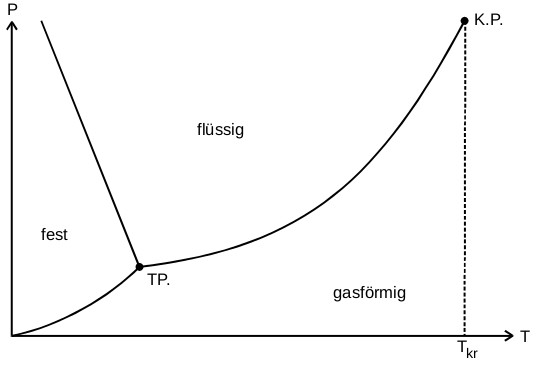
\includegraphics[width=0.75\linewidth]{./images/zustand.jpg}
    \caption{Zustandsdiagramm von Wasser \cite{V203}}
    \label{fig:1}
\end{figure}
\flushleft{An\;}\justifying dem Beispiel für das Zustandsdiagramm von Wasser lassen sich die drei
charakteristischen Phasen an den drei abgegrenzten Gebieten gut unterscheiden.
Der Punkt TP. stellt dabei den Tripelpunkt von Wasser dar, an dem alle drei Aggregatszustände
koexistieren können. Der Punkt K.P. hingegen beschreibt den kritischen Punkt, an dem sich
die Zustände gasförmig und flüssig nicht mehr unterscheiden lassen. Die Verbindungskurve
des Tripelpunktes mit dem kritischen Punkt wird dabei als Dampfdruckkurve bezeichnet und
stellt den Zustand dar, in dem zwei Phasen koexistieren können.
Für den Fall von Wasser sind das flüssig und gasförmig.
Bei einer Änderung der Temperatur oder des Druckes kann sich der Aggregatszustand eines
Stoffes ändern. \\
Dabei wird im folgenden die Phasenänderung von flüssig zu gasförmig betrachtet.
Bei der Verdampfung wird im Allgemeinen eine neue Größe eingeführt, die Verdampfungswärme $L$.
Sie beschreibt die benötigte Energiemenge, um ein bestimmtes Volumen an Flüssigkeit vollständig
verdampfen zu lassen. Mit der Verdampfungswärme wird ebenfalls der Verlauf der Dampfdruckkurve beschrieben.
Die Verdampfungswärme bildet damit eine charakteristische Eigenschaft von verschiedenen Stoffen,
welche von der Temperatur abhängt.\\
Zur Berechnung der Verdampfungswärme werden mikroskopische Vorgänge betrachtet. Bei diesen
wird festgestellt, dass der Druck des Dampfes nicht durch die allgemeine Gasgleichung \cite{V203}
\begin{align}
    pV=RT \label{eq:1} \quad \text{R:=allgemeine Gaskonstante}
\end{align}
beschrieben werden kann. \\
Daher wird die molare Verdampfungswärme, welche die Verdampfung von einem Mol der Flüssigkeit
beschreibt, durch folgende Differentialgleichung beschrieben \cite{V203}:
\begin{align}
    \left(V_D - V_F\right)dp=\frac{L}{T} \; dT \label{eq:2}.
\end{align}
$V_D$ und $V_F$ sind dabei das Volumen des Dampfes und der Flüssigkeit, T die Temperatur und p der Dampfdruck,
wobei $V_D$ mit der Gleichung \cite{V203}
\begin{align}
    \left(p+\frac{a}{V^2}\right)V=RT \qquad \text{mit} \qquad a=0,9 \;\frac{Joule\,m^3}{Mol^2} \label{eq:3}
\end{align}
bestimmt werden kann.
Die Gleichung \eqref{eq:2} wird auch als Clausius-Clapeyronsche Gleichung bezeichnet.
Die Bestimmung der allgemeinen Lösung der Differentialgleichung ist schwierig. \\
Daher werden einige Näherungen für den Temperaturbereich $T \ll T_{kr}$ gemacht.
Zum einen ist $V_F$ gegnüber $V_D$ vernachlässigbar.
Zum anderen kann $V_D$ durch die ideale Gasgleichung beschrieben werden \cite{V203}:
\begin{align}
    V_D(p,T)=R \; \frac{T}{p} \label{eq:4}.
\end{align}
Außerdem ist L konstant, wodurch sich für den Druck p die Formel \cite{V203}
\begin{align}
    \ln(p)=- \frac{L}{R} \frac{1}{T}+const \label{eq:5}
\end{align}
ergibt.
\newpage

% Fehlerrechnung %%%%%%%%%%%%%%%%%%%%%%%%%%%%%%%%%%%%%%%%%%%%%%%%%%%%%%%%%%%%%%%%%%%%%%%%%%%%%%%%%%%%%%%%%%%%%%%%%%%%%%%%%%%%%%%%%%%%%%%%%%%%%%%%%%%%%%%%%%%%%%%%%%%%%%%%%%%%%%%%%%%%%%%%%%%%%%%%%%%%%%%%%%%%%%%%%%%%%%

\section{Fehlerrechnung}\justifying
Für die Berechnung von Messunsicherheiten werden in diesem Protokoll folgende Formeln
verwendet:
\begin{subequations} \label{eq:6}
\begin{align} 
\intertext{Zur Bestimmung eines Mittelwertes wird folgende Formel benutzt:
}
    \overline{x} &= \frac{1}{N}\sum_{i=1}^{N} x_i \label{eq:6a}
\intertext{Zur Bestimmung der Messunsicherheit bei Mittelwerten wird mit der Formel
}
    \Delta\overline{x} &= \frac{1}{\sqrt{N}} \sqrt{\frac{1}{1-N} \sum_{i=1}^{N} (x_i - \overline{x})^2} \label{eq:6b},
\intertext{gearbeitet und die Gaußsche Fehlerfortpflanzung wird mit
}
    \Delta f &= \sqrt{\sum_{i=1}^{N} \left( \frac{\delta f}{\delta x_i} \right)^2 \cdot (\Delta x_i)^2} \label{eq:6c}
\intertext{berechnet. Um Ausgleichsgeraden und ihre Parameter zu bestimmen, werden folgende Formeln verwendet:
}
    y &= m \cdot x + b \label{eq:6d} \\ 
    m &= \frac{\overline{xy} - \overline{x} \cdot \overline{y}}{\overline{x^2} - {\overline{x}}^2} \label{eq:6e}\\
    b &= \frac{\overline{y} \cdot \overline{x^2} - \overline{xy} \cdot \overline{x}}{\overline{x^2} - {\overline{x}}^2} \label{eq:6f}
\end{align}
\end{subequations}
\newpage

% Versuchsaufbau + Versuchsdurchführung %%%%%%%%%%%%%%%%%%%%%%%%%%%%%%%%%%%%%%%%%%%%%%%%%%%%%%%%%%%%%%%%%%%%%%%%%%%%%%%%%%%%%%%%%%%%%%%%%%%%%%%%%%%%%%%%%%%%%%%%%%%%%%%%%%%%%%%%%%%%%%%%%%%%%%%%%%%%%%%%%%%%%%%%%%%%%%%%%%%%%%%%%%%%%%%%%%

% unter 1 bar ----------------------------------------------------------------------------------------------------------------------------------------------------------------------------------------------------------------------------------

\section{Versuchsaufbau und Versuchsdurchführung}\justifying

\flushleft{Aufbau\;}\justifying und Durchführung für den Druckbereich unter $\SI{1}{\bar}$:

\flushleft{Benötigt\;}\justifying werden: \textit{Eine Wasserstrahlpumpe, ein Absperrhahn, eine Woulffsche Flasche, ein Belüftungsventil, ein Drosselventil, ein Manometer, 
einen Rückflußkühler, zwei Flüssigkeitsthermometer, einen Mehrhalskolben, eine regelbare Heizhaube und destilliertes und entgastes Wasser.}

\flushleft{Für\;}\justifying die Temperatur- und Druckermittelung unter $\SI{1}{\bar}$ wird der Versuch, wie in Abbildung \ref{fig:2} dargestellt,
aufgebaut.

\begin{figure}
    \centering
    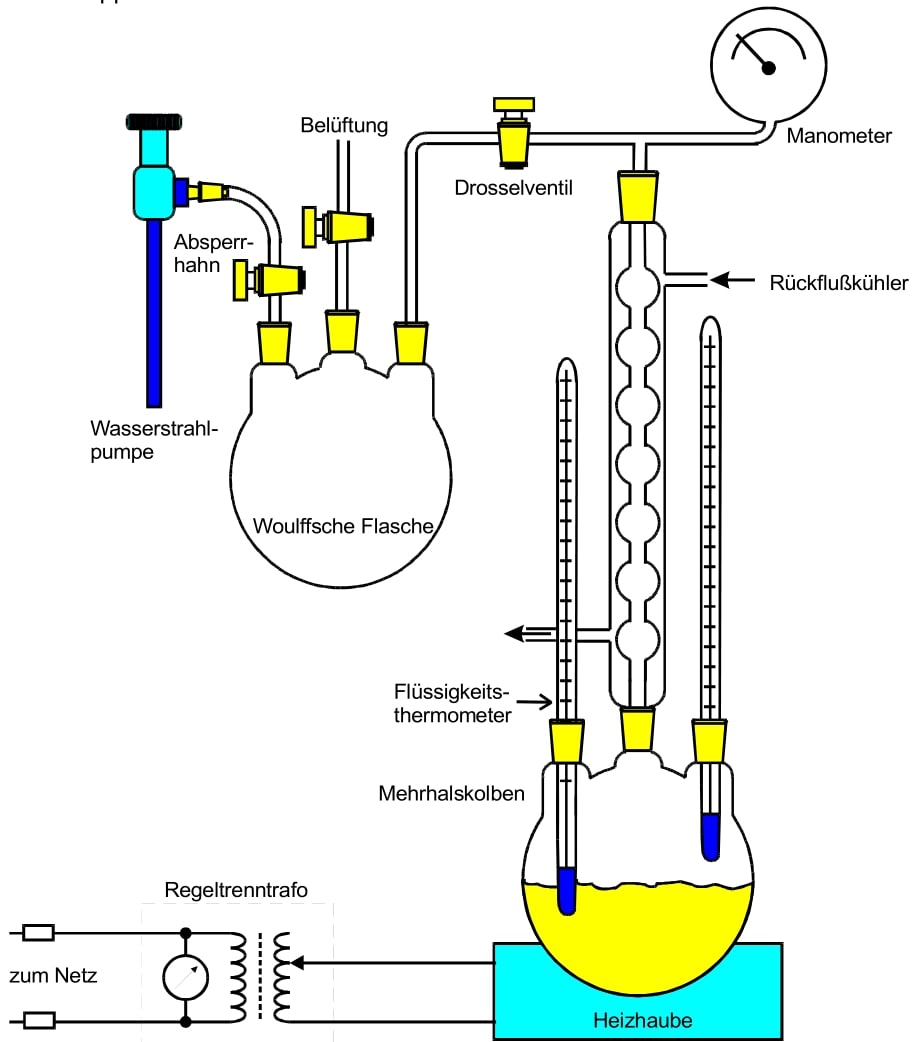
\includegraphics[width=0.75\linewidth]{./images/k1bar.jpg}
    \caption{Versuchsaufbau für Druckbereich $\leq \SI{1}{\bar}$ \cite{V203}}
    \label{fig:2}
\end{figure}
\newpage

\flushleft{Zu\;}\justifying Beginn muss der Mehrhalskolben evakuiert werden. Dazu wird das Belüftungsventil geschlossen und der Absperrhahn und
das Drosselventil geöffnet. Anschließend wird die Wasserstrahlpumpe eingeschaltet. Nun wird der interne Druck des Aufbaus mit dem Manometer
beobachtet bis der Druck auf ca. $\SI{60}{\milli\bar}$ gesunken ist. Ist dies eingetreten, wird das Drosselventil geschlossen, die Heizhaube
eingeschaltet und Wasser durch den Rückflußkühler geleitet. Gleichzeitig wird außerdem die Wasserstrahlpumpe abgeschaltet. Mit dem rechten
Thermometer wird nun die Temperatur des Gases gemessen. Hier misst das Gas eine Zimmertemperatur von $\SI{21}{\celsius}$. Es wird für jeden 
weiteren ganzzahligen Grad der entsprechende Druck dem Manometer entnommen. Dieser Prozess wird wiederholt, bis in dem Mehrhalskolben der Druck 
auf $\SI{1}{\bar}$ ($\SI{1000}{\milli\bar}$) gestiegen ist. Abschließend wird die Heizhaube ausgeschaltet und alle Ventile geöffnet.  

% über 1 bar ----------------------------------------------------------------------------------------------------------------------------------------------------------------------------------------------------------------------------------

\flushleft{Aufbau\;}\justifying und Durchführung für den Druckbereich über $\SI{1}{\bar}$:

\flushleft{Benötigt\;}\justifying werden: \textit{Ein Flüssigkeitsthermometer, ein Drucksensor, ein analoges Manometer, ein U-Rohr, ein Metallzylinder, eine Heizwicklung 
(hier ein elektrischer Heizkörper).}

\flushleft{Für\;}\justifying die Temperatur- und Druckermittelung über $\SI{1}{\bar}$, wird der Versuch ähnlich zur Abbildung \ref{fig:3} aufgebaut. 
Hier wird allerdings die Kühlschale weggelassen und die Heizwicklung durch einen, unter den Zylinder befindlichen, Heizkörper ersetzt. 

\begin{figure}[H]
    \centering
    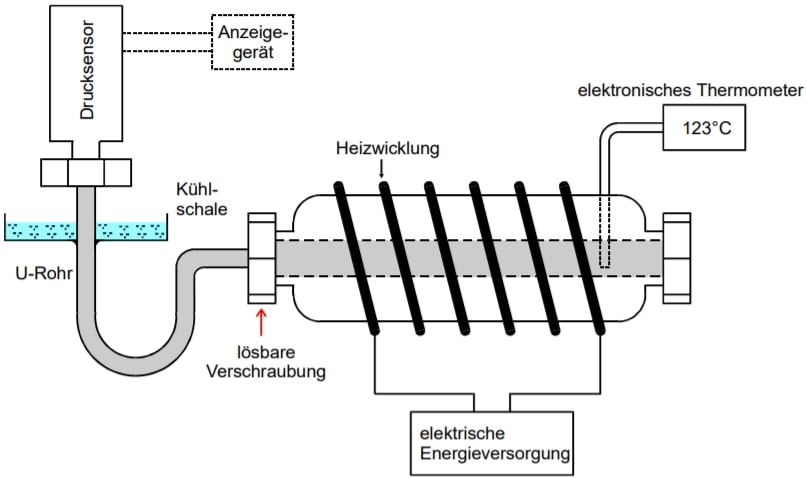
\includegraphics[width=\linewidth]{./images/g1bar.jpg}
    \caption{Versuchsaufbau für Druckbereich $\geq \SI{1}{\bar}$ \cite{V203}}
    \label{fig:3}
\end{figure}

\flushleft{Zuerst\;}\justifying wird der Heizkörper eingeschaltet. Anschließend wird die Temperatur für jeden halben $\SI{}{\bar}$ vom Thermometer
abgelesen. Dies wird wiederholt, bis das Manometer $\SI{15}{\bar}$ anzeigt. Abschließend wird der Heizkörper ausgeschaltet.

% Auswertung %%%%%%%%%%%%%%%%%%%%%%%%%%%%%%%%%%%%%%%%%%%%%%%%%%%%%%%%%%%%%%%%%%%%%%%%%%%%%%%%%%%%%%%%%%%%%%%%%%%%%%%%%%%%%%%%%%%%%%%%%%%%%%%%%%%%%%%%%%%%%%%%%%%%%%%%%%%%%%%%%%%%%%%%%%%%%%%%%%%%%%%%%%%%%%%%%%

\section{Auswertung}

\subsection{Druckbereich für $p < \SI{1}{bar}$}

\flushleft{Die\;}\justifying für den Bereich kleiner als ein Bar aufgenommenen Messwerte sind in der folgenden Tabelle \ref{tab:1} aufgetragen:

\begin{table}
    \centering
    \input{table_k1bar.tex}
    \caption{Temperatur für den Druckbereich $\leq \SI{1}{\bar}$}
    \label{tab:1}
\end{table}

\flushleft{Mithlife\;}\justifying der Messwerte aus Tabelle \ref{tab:1} wird der folgende Graph \ref{fig:4} des logarithmischen Dampfdruckes und
der reziproken absoluten Temperatur erstellt. Der logarithmische Druck $\log{p}$ und die reziproke absolute $\sfrac{1}{T}$ 
Temperatur werden mit den entsprechenden Werten aus Tabelle \ref{tab:1} bestimmt.
\newpage

\flushleft{Die\;}\justifying Parameter $m$ und $b$ werden mit dem Python Befehl polyfit \cite{uncertainties} bestimmt. Die Verdampfungswärme $L$ lässt sich mit dem 
negativen Parameter $m$ und der Gaskonstante $R$ berechnen. Für die Gaskonstante $R$ wird der Befehl const.R aus der Scipybibliothek \cite{scipy} verwendet.
Aufgrund des Koeffizientenvergleichs der Geradengleichung mit Formel \eqref{eq:5} ergibt sich für $L = -m \cdot R$.

\flushleft{Die\;}\justifying für den Graphen \ref{fig:4} relevanten Parameter lauten wie folgt:

\begin{subequations} \label{eq:7}
\begin{align}
    m &= \text{\input{m_plotk1b.tex}} \label{eq:7a}\\
    b &= \text{\input{b_plotk1b.tex}} \label{eq:7b}\\
    L &= \text{\input{Lk1b.tex}} \label{eq:7c}
\end{align}
\end{subequations}

\begin{figure}[H]
    \centering
    \includegraphics[width=\textwidth]{./build/plotk1b.pdf}
    \caption{Plot für Druckbereich $\leq \SI{1}{\bar}$}
    \label{fig:4}
\end{figure}

\flushleft{Die\;}\justifying Verdampfungswärme $L$ \eqref{eq:7c} wird nun von der äußeren Verdampfungswärme $L_a$ abgezogen um $L_i$ zu 
erhalten. $L_a$ erhält man aus der allgemeinen Gasgleichung \eqref{eq:1}, wenn für die Temperatur $T = \SI{373}{\kelvin}$ eingesetzt wird. 
Daraus folgt $L_a = R \cdot T$. Wird nun $L_i = L - L_a$ berechnet, folgt:

\begin{subequations} \label{eq:8}
\begin{align}
    L_a &= \text{\input{L_a.tex}} \label{eq:8a}\\
    L_i &= \text{\input{L_i.tex}} \label{eq:8b}
\end{align}
\end{subequations}

\subsection{Druckbereich für $p > \SI{1}{bar}$}

Die Tabelle für den Versuch im Druckbereich $p> \SI{1}{\bar} $ sieht wie folgt aus:

\begin{table}[H]
    \centering
    \input{table_g1bar.tex}
    \caption{Temperatur für den Druckbereich $\geq \SI{1}{\bar}$}
    \label{tab:2}
\end{table}

\flushleft{Mithilfe\;}\justifying der Messwerte aus der Tabelle \ref{tab:2} wird ein Polynom
3. Grades für den Druck in Abhängigkeit der Temperatur bestimmt

\begin{align}
    p(T)= aT^3 +bT^2 +cT +d \label{eq:9}
\end{align}
mit den Fitparametern
\begin{subequations} \label{eq:10}
\begin{align}
    a &= \text{\input{parg1b_a.tex}}, \label{eq:10a}\\
    b &= \text{\input{parg1b_b.tex}}, \label{eq:10b}\\
    c &= \text{\input{parg1b_c.tex}} \quad \text{und} \label{eq:10c}\\
    d &= \text{\input{parg1b_d.tex}}. \label{eq:10d}
\end{align}
\end{subequations}
Die Fitparameter werden mit der Funktion polyfit() von Numpy \cite{numpy} berechnet.
Mit diesem Polynom wird durch Ableiten, einsetzen und mitteln der Quotient $\overline{\frac{dp}{dT}}$ bestimmt:
\begin{align} 
    \frac{dp}{dT}&= 3\cdot a T^2+2\cdot b T+c \label{eq:11}\\
    \overline{\frac{dp}{dT}}&= \text{\input{dpdT.tex}} \label{eq:12}
\end{align}
Für die Berechnung des Dampfvolumens wird die Gleichung \eqref{eq:3} in eine 
quadratische Gleichung für das Volumen V umgeschrieben, mittels pq-Gleichung gelöst
und gemittelt:
\begin{subequations} \label{eq:13}
\begin{align}
    V_D&^2-\frac{RT}{p}\cdot V_D+\frac{a}{p}=0 \label{eq:13a}\\
    V_D&= \frac{RT}{2p} \pm \sqrt{\frac{R^2T^2}{4p^2} -\frac{a}{p} } \label{eq:13b}\\
    V_{D,+}&= \text{\input{VDplus.tex}} \label{eq:13c}\\
    V_{D,-}&= \text{\input{VDminus.tex}} \label{eq:13d}
\end{align}
\end{subequations}

\flushleft{Anschließend\;}\justifying wird die Verdampfungswärme gegen die Temperatur in einem Graphen aufgetragen:

\begin{figure}[H]
\begin{subfigure}{0.495\linewidth}
    \centering
    \includegraphics[width=\textwidth]{./build/plotg1bplus.pdf}
    \caption{Plot für die Temperaturabhängigkeit der Verdampfungswärme mit $V_{D,+}$}
    \label{fig:5a}
\end{subfigure}
\begin{subfigure}{0.495\linewidth}
    \centering
    \includegraphics[width=\textwidth]{./build/plotg1bminus.pdf}
    \caption{Plot für die Temperaturabhängigkeit der Verdampfungswärme mit $V_{D,-}$}
    \label{fig:5b}
\end{subfigure}
\caption{Plots für die Temperaturabhängigkeit\label{fig:5}}
\end{figure}

\flushleft{Die\;}\justifying Werte für die Dampfungswärme werden über die Formel \eqref{eq:2}  
\begin{align}
    L= V_D \cdot \frac{dp}{dT}\cdot T \qquad (V_F = 0) \label{eq:14}
\end{align}
sowie den berechneten Parametern \eqref{eq:12}, \eqref{eq:13c}, \eqref{eq:13d} und den Temperaturwerten aus Tabelle \ref{tab:2}.

\flushleft{Die\;}\justifying, mit polyfit \cite{numpy} berechneten,  Parameter der Ausgleichsgeraden lauten wie folgt:

\begin{subequations} \label{eq:15}
\begin{align}
    m_{+} &= \text{\input{Lg1b_mplus.tex}}  &m_{-} &=\text{\input{Lg1b_mminus.tex}}  \label{eq:15a}\\
    b_{+} &= \text{\input{Lg1b_bplus.tex}} &b_{+} &= \text{\input{Lg1b_bminus.tex}}  \label{eq:15b}
\end{align}
\end{subequations}
\newpage

% Diskussion %%%%%%%%%%%%%%%%%%%%%%%%%%%%%%%%%%%%%%%%%%%%%%%%%%%%%%%%%%%%%%%%%%%%%%%%%%%%%%%%%%%%%%%%%%%%%%%%%%%%%%%%%%%%%%%%%%%%%%%%%%%%%%%%%%%%%%%%%%%%%%%%%%%%%%%%%%%%%%%%%%%%%%%%%%%%%%%%%%%%%%%%%%%%%%%%%%

\section{Diskussion}

\flushleft{Der\;}\justifying Graph \ref{fig:4} stellt ein lineares Verhältniss zwischen dem Logarithmus des Drucks $\left( \log{p} \right)$ und 
der absoluten Temperatur $\left( \sfrac{1}{T} \cdot 10^{-3} \right)$. Die Messwerte liegen zum Großteil auf der Ausgleichsgeraden, wobei die letzten 
zehn Werte nach oben abweichen. Der Literaturwert der Verdampfungswärme liegt bei $\SI{40.7}{\kilo\joule\per\mole}$ \cite{Verdampfungswärme}, welcher
für die experimentell bestimmte Verdampfungswärme des Graphen \ref{fig:4} einen relativer Fehler von
\begin{equation}
    \frac{L_{Exp.} - L_{Lit.}}{L_{Lit.}} = \text{\input{Fehler_Lk1b.tex}} \label{eq:16}
\end{equation}

% Literatur %%%%%%%%%%%%%%%%%%%%%%%%%%%%%%%%%%%%%%%%%%%%%%%%%%%%%%%%%%%%%%%%%%%%%%%%%%%%%%%%%%%%%%%%%%%%%%%%%%%%%%%%%%%%%%%%%%%%%%%%%%%%%%%%%%%%%%%%%%%%%%%%%%%%%%%%%%%%%%%%%%%%%%%%%%%%%%%%%%%%%%%%%%%%%%%%%%

\newpage
\printbibliography

\end{document}
